%\documentclass[t,11pt,handout,usenames,dvipsnames]{beamer}
\documentclass[t,11pt,usenames,dvipsnames]{beamer}
%\documentclass[t,mathserif,11pt]{beamer} 
%\usetheme{Berlin}
%\usecolortheme{seahorse}
\usefonttheme{serif}
\usetheme{CambridgeUS}
\usecolortheme{rose}
\usecolortheme{dolphin}

%\usefonttheme[onlymath]{serif}

\setbeamertemplate{itemize items}[square]
\setbeamertemplate{itemize subitem}[circle]
\setbeamertemplate{itemize subsubitem}[triangle]

\setbeamertemplate{enumerate items}[default]




\usepackage{verbatim}
%\usepackage{multirow}
\usepackage[normalem]{ulem}

%\newcommand\hmmax{0}
\usepackage{hyperref}
%\usepackage[abbrev]{amsrefs}

%\usepackage{bbold}
%\usepackage{bbm}
%\def\mathbb{\mathbbm}
\usepackage{amssymb}
\usepackage{amsmath}
%\usepackage{unicode-math}
%\usepackage{amsthm}
\usepackage{graphicx}
\usepackage{braket}
%\usepackage{paralist}
%\usepackage{rotating}
%\usepackage{arydshln}

%\usepackage{color}
\usepackage{xcolor}
%\usepackage[all,color]{xy}
%\UseCrayolaColors

%\usepackage{mathabx}
\usepackage{mathrsfs}
%\usepackage{MnSymbol}
%\usepackage{mathbbol}
%\usepackage{psnfss}



\usepackage{youngtab}
\Yautoscale1
\Yvcentermath1

\usepackage[centertableaux,smalltableaux]{ytableau}

%\usepackage{cleveref}

\theoremstyle{plain}
\newtheorem{thm}{Theorem}
\newtheorem{claim}{Claim}
\newtheorem{conj}{Conjecture}

%\newtheorem{lemA}[thmA]{Lemma}
%\newtheorem{propA}[thmA]{Proposition}
%\newtheorem{corA}[thmA]{Corollary}
%\newtheorem{thm}[subsection]{Theorem}
%\newtheorem{lemma}{Lemma}
\newtheorem{prop}{Proposition}
\newtheorem{cor}{Corollary}
%\newtheorem*{prop*}{Proposition}

\theoremstyle{definition}
\newtheorem{defn}{Definition}



\definecolor{refkey}{gray}{.3}
\definecolor{labelkey}{gray}{.3}


% \def\cone{\ding{172}}
% \def\ctwo{\ding{173}}
% \def\cthree{\ding{174}}
% \def\cfour{\ding{175}}
% \def\cfive{\ding{176}}



\newcommand{\mjjc}[1]{\marginpar{\color{green}\tiny #1 \mbox{--ma}}}


\newcommand{\rk}{\mathrm{rk}}
\newcommand{\cqq}{\mathscr{D}}
\newcommand{\Sym}{\mathrm{Sym}}
\newcommand{\rSp}{\mathrm{Sp}}
\newcommand{\rsym}{\mathrm{sym}}
\newcommand{\rO}{\mathrm{O}}
\newcommand{\SO}{\mathrm{SO}}
\newcommand{\rskew}{\mathrm{skew}}
\newcommand{\fraksp}{\mathfrak{sp}}
\newcommand{\frakso}{\mathfrak{so}}
\newcommand{\frakm}{\mathfrak{m}}
\newcommand{\frakp}{\mathfrak{p}}
\newcommand{\pr}{\mathrm{pr}}
\newcommand{\rhopst}{\rho'^*}
\newcommand{\Rad}{\mathrm{Rad}}
\newcommand{\Res}{\mathrm{Res}}
\newcommand{\Hol}{\mathrm{Hol}}
\newcommand{\AC}{\mathrm{AC}}
\newcommand{\AV}{\mathrm{AV}}
\newcommand{\VC}{\mathrm{V}_\bC}
\newcommand{\bfv}{\mathbf{v}}
\newcommand{\depth}{\mathrm{depth}}
\newcommand{\wtM}{\widetilde{M}}
\newcommand{\wtMone}{{\widetilde{M}^{(1,1)}}}

\newcommand{\nullpp}{N(\fpp'^*)}
\newcommand{\nullp}{N(\fpp^*)}
\newcommand{\Aut}{\mathrm{Aut}}



\newcommand{\bfone}{\mathbf{1}}
\newcommand{\bbone}{\mathbb{1}}




\newcommand{\sfVprime}{\mathsf{V}^\prime}
\newcommand{\sfVdprime}{\mathsf{V}^{\prime \prime}}
\newcommand{\gminusone}{\mathfrak{g}_{-\frac{1}{m}}}

\newcommand{\eva}{\mathrm{eva}}

\newcommand\iso{\xrightarrow{
\,\smash{\raisebox{-0.65ex}{\ensuremath{\scriptstyle\sim}}}\,}}

\def\tmu{\tilde{\mu}}

\def\tr{\mathrm{tr}}
\def\trD{{\tr_{D/F}}}
\def\trF{{\tr_F}}

\def\Ueven{{U_{\rm{even}}}}
\def\Uodd{{U_{\rm{odd}}}}
\def\ttau{\tilde{\tau}}
\def\Wcp{W}
\def\Kur{{K^{\mathrm{u}}}}


\providecommand{\bcN}{{\overline{\cN}}}
\providecommand{\bcO}{{\overline{\cO}}}

\def\Mpii{M'^{(1,1)}}
\def\Mptz{M'^{(2,0)}}
\def\Mpzt{M'^{(0,2)}}
\def\mpii{\fmm'^{(1,1)}}
\def\mptz{\fmm'^{(2,0)}}
\def\mpzt{\fmm'^{(0,2)}}
\def\bcOp{\overline{\cO'}}

\def\frakN{\mathfrak{N}}
\def\topform{\mbox{$\bigwedge^{\! \mathrm{top} \, }$}}

\def\barxi{{\overline{\xi}}}
\def\Stab{{\rm Stab}}
\def\ad{{\rm ad}}
\def\Ad{{\rm Ad}}
\def\id{{\rm id}}
\def\sgn{{\rm sgn}}
\def\gcd{{\rm gcd}}

\makeatletter
\def\inn#1#2{\left\langle 
\def\ta{#1}\def\tb{#2}
\ifx\ta\@empty{\;} \else {\ta}\fi ,
\ifx\tb\@empty{\;} \else {\tb}\fi
\right\rangle} 
\makeatother

\def\innw#1#2{\inn{#1}{#2}_{W}}
\def\innv#1#2{\inn{#1}{#2}_{V}}
\def\innvp#1#2{\inn{#1}{#2}_{V'}}
\def\innGa#1#2{\inn{#1}{#2}_{\Gamma}}
\def\innGap#1#2{\inn{#1}{#2}_{\Gamma'}}

\def\abs#1{\left|{#1}\right|}
\def\norm#1{{\left\|{#1}\right\|}}



\def\mydefhat#1{\expandafter\def\csname hat#1\endcsname{\hat{#1}}}
\def\mydefwh#1{\expandafter\def\csname wh#1\endcsname{\widehat{#1}}}
\def\mydeft#1{\expandafter\def\csname t#1\endcsname{\tilde{#1}}}
\def\mydefr#1{\expandafter\def\csname r#1\endcsname{\mathrm{#1}}}
\def\mydefb#1{\expandafter\def\csname b#1\endcsname{\mathbb{#1}}}
\def\mydefwt#1{\expandafter\def\csname wt#1\endcsname{\widetilde{#1}}}
\def\mydeff#1{\expandafter\def\csname f#1\endcsname{\mathfrak{#1}}}
\def\mydefbf#1{\expandafter\def\csname bf#1\endcsname{\mathbf{#1}}}
\def\mydefc#1{\expandafter\def\csname c#1\endcsname{\mathcal{#1}}}
\def\mydefsf#1{\expandafter\def\csname sf#1\endcsname{\mathsf{#1}}}
\def\mydefs#1{\expandafter\def\csname s#1\endcsname{\mathscr{#1}}}
\def\mydefcks#1{\expandafter\def\csname cks#1\endcsname{{\check{
\csname s#1\endcsname}}}}
\def\mydefck#1{\expandafter\def\csname ck#1\endcsname{{\check{
#1}}}}

\def\mydefbfdowncase#1{
\expandafter\def\csname bf#1#1\endcsname{\mathbf{#1}}
}
\def\mydefckdowncase#1{
\expandafter\def\csname ck#1#1\endcsname{\check{#1}}
}
\def\mydefrmdowncase#1{
\expandafter\def\csname r#1#1\endcsname{\mathrm{#1}}
}
\def\mydefsfdowncase#1{
\expandafter\def\csname sf#1#1\endcsname{\mathsf{#1}}
}
\def\mydeffdowncase#1{
\expandafter\def\csname f#1#1\endcsname{\mathfrak{#1}}
}

\def\doAZ#1{#1A #1B #1C #1D #1E #1F #1G #1H #1I #1J #1K #1L 
#1M #1N #1O #1P #1Q #1R #1S #1T #1U #1V #1W #1X #1Y #1Z}
\def\doaz#1{#1a #1b #1c #1d #1e #1f #1g #1h #1i #1j #1k #1l 
#1m #1n #1o #1p #1q #1r #1s #1t #1u #1v #1w #1x #1y #1z}

\doAZ{\mydefsf}
\doAZ{\mydeft}
\doAZ{\mydefwh}
\doAZ{\mydefhat}
\doAZ{\mydefr}
\doAZ{\mydefwt}
\doAZ{\mydeff}
\doAZ{\mydefb}
\doAZ{\mydefbf}
\doAZ{\mydefc}
\doAZ{\mydefs}
\doAZ{\mydefck}
\doAZ{\mydefcks}

\doaz{\mydefbfdowncase}
\doaz{\mydeffdowncase}
\doaz{\mydefrmdowncase}
\doaz{\mydefsfdowncase}
\doaz{\mydefckdowncase}




\def\wtGL{\widetilde{\GL}}
\def\wtSp{\widetilde{\rSp}}
\def\tSp{\tilde{\rSp}}


\def\trho{{\widetilde{\rho}}}
\def\tiota{{\widetilde{\iota}}}
\def\biota{{\overline{\iota}}}



\def\GL{\mathrm{GL}}
\def\wtSp{\widetilde{\mathrm{Sp}}}
\def\fsp{{\mathfrak{sp}}}
\def\fgl{{\mathfrak{gl}}}
\def\fsl{{\mathfrak{sl}}}
\DeclareMathOperator{\Wh}{Wh}
\DeclareMathOperator{\WF}{WF}

\def\Id{\mathrm{Id}}
\def\Ann{{\mathrm{Ann}\,}}
\def\Ker{{\rm Ker}\,}
\def\Lie{{\rm Lie}}
\def\Im{{\rm Im\,}}
\def\Hom{{\rm Hom}}
\def\End{{\rm End}}
\def\Mat{{\rm Mat}}
\def\Ind{{\rm Ind}}
\def\ind{{\rm ind}}
\def\Spec{{\rm Spec\,}}
\def\Supp{\mathrm{Supp}}
\def\Sym{\mathrm{Sym}}
\def\Alt{\mathrm{Alt}}
\def\Gr{\mathrm{Gr\,}}
\def\codim{\mathrm{codim}}
\def\rank{\mathrm{rank}}
\def\Gal{\mathrm{Gal}}

\def\cAV{{\cA\cV}}
\def\supp{{\rm{supp}\,}}
\def\wtMoo{{{\wtM^{(1,1)}}}}

\def\nosizesub#1#2{{{#1}_{\makebox[0pt][l]{$\scriptstyle {#2}$}}}}

% editing macros. 
\long\def\mjj#1{{{\color{magenta}#1}}}
\long\def\delete#1{}
\long\def\mjjd#1#2{{\color{blue}#1 \sout{#2}}}

\newcommand{\trivial}[2][]{\if\relax\detokenize{#1}\relax
{\green {\medskip The following is trivial. } #2}
\else 
\ifx#1h\relax  \else {\red Wrong argument!} \fi
\fi
}


\def\floor#1{{\lfloor #1 \rfloor}}
\def\ceil#1{{\lceil #1 \rceil}}
\def\foo{{\mathfrak{o}}}
\def\sV{{\mathscr{V}}}
\def\tjj{{\tilde{j}}}
\def\wtA{{\widetilde{A}}}
\def\iinn#1#2{\ll#1,#2\gg}
\def\fF{{\mathfrak{F}}}
\def\fM{{\mathfrak{M}}}
\def\Hom{{\mathrm{Hom}}}

\def\tww{{\tilde{w}}}
\def\tgg{{\tilde{g}}}
\def\hG{{\hat{G}}}
\def\LG{{{}^LG}}
\def\LN{{{}^LN}}
\def\hn{{\hat{n}}}
\def\hns{{\hat{n}_s}}
\def\hnt{{\hat{n}_t}}

\def\fppC{\fpp_\bC}
\def\fppCp{\fpp'_{\bC}}


\def\sW{{\mathscr{W}}}
\def\Stab{{\mathrm{Stab}}}
\def\Mp{{\mathrm{Mp}}}
\def\Sp{{\mathrm{Sp}}}
\def\SL{{\mathrm{SL}}}
\def\Irr{{\mathrm{Irr}}}
\def\cX{{\mathcal{X}}}
\def\cW{{\mathcal{W}}}
\def\rG{{\mathrm{G}}}
\def\Unip{{\mathrm{Unip}}}
\def\Ch{{\mathrm{Ch}}}

\def\Xllp{{{\mathsf{X}}_{\lambda,\lambda'}}}
\def\Pil{{\pi_{\lambda,\check{\rho}}}}
\def\Pilp{{\pi'_{\lambda',\rho'}}}

\def\piSigma{{\pi_\Sigma}}
\def\piSigmap{{\pi'_{\Sigma'}}}
\def\piSigmapp{{\pi'_{\Sigma''}}}


\def\wteta{{\widetilde{\eta}}}
\def\wtpi{{\widetilde{\pi}}}
\def\tpiSigma{{\wtpi_\Sigma}}
\def\tpiSigmap{{\wtpi'_{\Sigma'}}}
\def\tpiSigmapp{{\wtpi'_{\Sigma''}}}

\def\Latto{{\mathrm{Latt^1}}}


\def\half{{\frac{1}{2}}}
\def\halfm{{\frac{m}{2}}}
\def\halfmm{{\frac{m-1}{2}}}
\def\fracmm{{\frac{1}{m}}}
\def\fracdmm{{\frac{1}{2m}}}

\def\cdt{{c}}
\def\bPsi{{\overline{\Psi}}}
\def\bpsi{{\overline{\psi}}}

\def\vG{{\overrightarrow{G}}}
\def\vrr{{\overrightarrow{r}}}
\def\vphi{{\overrightarrow{\phi}}}

\def\Cent#1#2{{\mathrm{Z}_{#1}({#2})}}

\def\bomega{{\overline{\omega}}}
\def\bomegaS{{\bomega_S}}
\def\bomegadgS{{\bomega_{\dgS}}}

%\def\cInd{{\mathrm{c-Ind}}}
\DeclareMathOperator{\cInd}{c-Ind}

\def\istar{{\filledstar}}
\def\mstar{{\medstar}}
\def\dstar{{\medstarofdavid}}

\def\skewinv{{\mathrm{skew-inv}}}
\def\btt{{\mathbbm{t}}}

\def\diagJ{{J^\triangle}}

\def\dd{{\rm{d}}}
\def\dalpha{{\dd\alpha}}
\def\dalphap{{\dd\alpha^\perp}}
\def\odalpha{\overline{\dd\alpha}}
\def\odalphap{\overline{\dd\alpha^\perp}}

\def\vol{{\mathrm{vol}}}

\def\Jump{{\mathrm{Jump}}}

\def\CO{\cO}
\def\bTheta{\overline{\Theta}}
\def\ckcO{{\check{\cO}}}
\def\ckfgg{{\check{\fgg}}}
\def\ckfgl{{\check{\fgl}}}
\def\ckGamma{{\check{\Gamma}}}
\def\ckww{{\check{w}}}
\def\ckD{{\check{D}}}

\def\sspan{{\mathrm{Span}}}

\def\dbK{{\breve{K}}}
\def\dbKp{{\dbK_+}}
\def\dbKzp{{\dbK_{0^+}}}
\def\dbpsi{{\breve{\psi}}}
\def\dbrho{{\breve{\rho}}}
\def\dbkappa{{\breve{\kappa}}}
\def\dbeta{{\breve{\eta}}}

\def\TTidx#1#2{\,{}^{#1}\hspace{-0.1em}#2}

\def\mydefTT#1#2#3{
\expandafter\def\csname ii#3{#1}\endcsname{\TTidx{i}{#2{#1}}}
\expandafter\def\csname zz#3{#1}\endcsname{\TTidx{0}{#2{#1}}}
\expandafter\def\csname ll#3{#1}\endcsname{\TTidx{l}{#2{#1}}}
\expandafter\def\csname aa#3{#1}\endcsname{\TTidx{a}{#2{#1}}}
\expandafter\def\csname bb#3{#1}\endcsname{\TTidx{b}{#2{#1}}}
\expandafter\def\csname oo#3{#1}\endcsname{\TTidx{1}{#2{#1}}}
\expandafter\def\csname ss#3{#1}\endcsname{\TTidx{\boxslash}{#2{#1}}}
\expandafter\def\csname dg#3{#1}\endcsname{\TTidx{\boxbackslash}{#2{#1}}}
}
\def\usecsname#1{\csname #1\endcsname}
\def\useLetter#1{#1}
\def\usedbletter#1{#1#1}

\def\Vp{V'}
\def\sLp{\sL'}
\def\Sigmap{\Sigma'}
\def\fggp{\fgg'}

\mydefTT{sB}{\usecsname}{\useLetter}
\mydefTT{Sigma}{\usecsname}{\useLetter}
\mydefTT{Sigmap}{\usecsname}{\useLetter}
\mydefTT{Gamma}{\usecsname}{\useLetter}
\mydefTT{Omega}{\usecsname}{\useLetter}
\mydefTT{phi}{\usecsname}{\useLetter}
\mydefTT{eta}{\usecsname}{\useLetter}
\mydefTT{kappa}{\usecsname}{\useLetter}
\mydefTT{dbkappa}{\usecsname}{\useLetter}
\mydefTT{bomega}{\usecsname}{\useLetter}
\mydefTT{rho}{\usecsname}{\useLetter}
\mydefTT{dbrho}{\usecsname}{\useLetter}
\mydefTT{bfbb}{\usecsname}{\useLetter}
\mydefTT{sL}{\usecsname}{\useLetter}
\mydefTT{sLp}{\usecsname}{\useLetter}
\mydefTT{G}{\useLetter}{\useLetter}
\mydefTT{K}{\useLetter}{\useLetter}
\mydefTT{W}{\useLetter}{\useLetter}
\mydefTT{S}{\useLetter}{\useLetter}
\mydefTT{V}{\useLetter}{\useLetter}
\mydefTT{Vp}{\usecsname}{\useLetter}
\mydefTT{dbK}{\usecsname}{\useLetter}
\mydefTT{dbG}{\usecsname}{\useLetter}
\mydefTT{End}{\usecsname}{\useLetter}

\mydefTT{x}{\useLetter}{\usedbletter}
\mydefTT{v}{\useLetter}{\usedbletter}
\mydefTT{w}{\useLetter}{\usedbletter}
\mydefTT{fgg}{\usecsname}{\useLetter}
\mydefTT{fggp}{\usecsname}{\useLetter}


\def\zzll{\ell}

\def\bbsSB{\sS(\bbsB_0)}
\def\aasSB{\sS(\aasB_0)}
\def\iisSB{\sS(\iisB_0)}
\def\ssdbkappa{\TTidx{\boxslash}{\dbkappa}}

\def\ssbasB{\TTidx{\boxslash}{\sB^{ba}}}
\def\ssabsB{\TTidx{\boxslash}{\sB^{ab}}}
\def\ssiota{\TTidx{\boxslash}{\iota}}

\def\ssbabfbb{\TTidx{\boxslash}{\bfbb^{ba}}}
\def\ssabbfbb{\TTidx{\boxslash}{\bfbb^{ab}}}


\def\ssbaW{\TTidx{\boxslash}{W^{ba}}}
\def\ssabW{\TTidx{\boxslash}{W^{ab}}}

\def\ggs{\fgg_{x,s}}
\def\ggsp{\fgg'_{x',s}}
\def\ggss{\fgg_{x,s:s^+}}
\def\ggssp{\fgg'_{x',s:s^+}}


\def\nuD{{\nu_D}}
\def\nuF{{\nu_F}}
\def\fooD{{\foo_D}}
\def\fppD{{\fpp_D}}
\def\fffD{{\fff_D}}

\def\tkappa{{\widetilde{\kappa}}}
\def\tpsi{{\widetilde{\psi}}}

\def\sfGz{\sfG^0_x}
\def\sfGzp{\sfG'^0_{x'}}

\def\MM{\sfM}
\def\MMp{\sfM'}
\def\Nil{\mathrm{Nil}}

\def\barX{\bar{X}}

\def\psiGa{\psi_\Gamma}


\def\Sec#1{\S~#1}

\def\blue{\color{blue}}
\def\gray{\color{gray}}
\def\red{\color{red}}
\def\lblue{\color{blue}}

\def\vV{\bfV^\vee}
\def\bSb{\bS(\bfbb)}
\def\vcO{\cO^\vee}


\def\bbF{\overline{\bF}}

\def\PBP{\mathrm{PBP}}
\def\LS{\mathrm{LS}}
\def\AOD{\mathrm{AOD}}

\def\gen#1{\langle #1 \rangle}

\let\oldemph\emph
\def\emph#1{\oldemph{\blue #1}}
%\def\emp#1{\blue #1}

\allowdisplaybreaks

\let\ytb=\ytableaushort

\setbeamertemplate{section in toc}[sections numbered]

\def\TTPG{
\begin{frame}[c]{}
    \tableofcontents[currentsection,hideallsubsections,subsubsectionstyle=hide]
\end{frame}
}

\usepackage{listings}
% \lstset{
%     basicstyle=\ttfamily\tiny,
%     keywordstyle=\color{black},
%     commentstyle=\color{white}, % white comments
%     stringstyle=\ttfamily, % typewriter type for strings
%     showstringspaces=false,
%     breaklines=true,
%     emph={Output},emphstyle=\color{blue},
% } 

\usepackage{tikz}
\usetikzlibrary{matrix,arrows,positioning,cd,backgrounds}
\usetikzlibrary{decorations.pathmorphing,decorations.pathreplacing}

\title[Uni. Repn.]{Unipotent representations \\
of real classical groups}

\author[Ma, Jia-Jun]{Ma, Jia-Jun\\[2em] 
(joint with Dan Barbasch, Binyong Sun and  Chengbo Zhu)
}

\institute[SJTU]{School of Mathematical Sciences\\
Shanghai Jiao Tong University}


%\setbeamercovered{invisible}
%\setbeamercovered{transparent}
\setbeamertemplate{headline}{}
\setbeamertemplate{navigation symbols}{}
\defbeamertemplate{footline}{my footline}{%
\vskip1pt%
%\hrule
%\makebox[0pt][l]{\,\insertsection}%
\hspace*{\fill}%\insertshorttitle\hspace*{\fill}%
%\hfill
\llap{\insertpagenumber\,/\,\insertpresentationendpage\,}
%\hspace*{\fill}
\hspace*{\fill}
}
%\setbeamertemplate{footline}[my footline]
\setbeamertemplate{footline}[frame number]
%\includeonlyframes{tt,DU}
%\includeonlyframes{CG,AC,EX}
%\includeonlyframes{CT}

%\usefonttheme[onlymath]{serif}
\usefonttheme{serif}

\begin{document}

\begin{frame}[plain,label=tt]
    
    \titlepage
    \vspace{-3em}
% \centering{
%     (Zhejiang University)
% }
\end{frame}


% \begin{frame}[c]{Outline}
    %   \tableofcontents[hideallsubsections,subsubsectionstyle=hide]
    % \end{frame}

\def\vgraph#1#2{\ensuremath{\vcenter{\hbox{\includegraphics[width=#1]{#2}}}}}
\def\hgraph#1#2{\ensuremath{\vcenter{\hbox{\includegraphics[height=#1]{#2}}}}}
\def\hhgraph#1#2#3{\ensuremath{\begin{array}{c}\text{#3}\\
        \hbox{\includegraphics[height=#1]{#2}}
        \end{array}}}
    \section{Motivation}

    \begin{frame}
      \frametitle{Reductive groups and its representation}
      \begin{itemize}[<+->]
        \item $\bfG$: a linear algebraic group: $\SL_{n}$, $\Sp_{2n}$, $\rO_{n}$,
              $G_{2}$, $F_{4}$, $E_{6}$, $E_{7}$, $E_{8}\cdots$.
        \item \emph{Question:} How to classify \emph{$\Irr(G)$} where $G= \bfG(k)$?
        \item The structure of $\Irr(G)$?
        \item Deligne-Lusztig: \emph{Jordan decomposition} (finite group, 1970s)
        \item[] Define dual group $\bfG^{*}$.
            E.g. $\Sp_{2n} = \bfG\leftrightsquigarrow \bfG^{*} = \SO_{2n+1}$\\
        \[
             \hhgraph{0.13\textwidth}{Lusztig}{Lusztig} \hspace{2em}
             \Irr(G) = \displaystyle \bigsqcup_{\text{s.s. class in } G^{*}} \cE(G, s).
             \hspace{2em}
             \hhgraph{0.13\textwidth}{Deligne}{Deligne}
            \]
        \item[] Lusztig's map to the unipotent packet.
        \[
          \cE(G,s)\xrightarrow{ 1-1 } \cE(G^{*}_{s},1)
        \]
      \end{itemize}
    \end{frame}

    \begin{frame}
      \frametitle{Representations of Real Lie groups}
      \begin{itemize}[<+->]
        \item Examples $G=\GL_{n}(\bR),\rU(p,q), \rO(p,q), \Sp(2n,\bR), \Mp(2n,\bR), \cdots$\\[-1em]
        \item[]\
              \vspace{-1em}
        \[
          \set{\text{discrete series}}\subset\set{\text{tempered}}
          \subset\set{\text{unitary}}\subset\Irr(G)
        \]
        \item Unitary dual of $\SL_{2}(\bR)$:
        \[
          \vgraph{0.6\textwidth}{unitary_sl2.png}
        \]
        \item \emph{Open problem:} Classify the unitary dual!
      \end{itemize}
    \end{frame}

    \def\vG{G^\vee}
    \begin{frame}
      \frametitle{Langlands and Arthur}
      \begin{itemize}[<+->]
        \item $W_{\bR} = \bC^{\times} \cup j\, \bC^{\times}$
        such that $jzj^{\, -1} = \overline{z}, j^{\, 2}=-1\in \bC^{\times}$.
        \item Langlands dual group ${}^{L}G = \vG \rtimes \braket{j}$. Eg:
        \[
          \Sp_{2n}(\bR)=G\longleftrightarrow \vG=\SO_{2n+1}(\bC)
        \]
        \item \emph{Langlands}
        \[
          \vgraph{0.12\textwidth}{Langlands.jpeg}
          \hspace{4em}
          \Irr(G)\xrightarrow{\text{\ finite to one\
            }} \set{\phi\colon W_{\bR}\rightarrow {}^{L}G}/\vG.
          \hspace{4em}
        \]
        \item \emph{Arthur: (Classical group, 2013)} $\Irr_{\text{temp}}(G) \subset \Irr_{A}(G)\subset
        \Irr_{\text{unit}}(G)$
        \[
          \vgraph{0.15\textwidth}{Arthur.jpg}
          \hspace{2em}
          \Irr_{A}(G)\xrightarrow{\text{\ finite to finite\
            }} \set{\psi\colon W_{\bR}\times \SL_{2}(\bC)\rightarrow {}^{L}G}/\vG.
        \]
      \end{itemize}
    \end{frame}


    \begin{frame}
      \frametitle{Arthur's unipotent representations}
      \begin{itemize}[<+->]
        \item $\psi:W_{\bR}\times \SL_{2}(\bC)\rightarrow {}^{L} G $
        \item Unipotent parameter $\Leftrightarrow$ $\psi|_{\bC^{\times}}=$ trivial
        \item[] $\Leftrightarrow$ nilpotent orbit of a real from of $\vG$.
        \item \vgraph{0.15\textwidth}{Arthur2.jpg}  \emph{Conjecture:} $\exists$ unipotent Arthur
        packets
        \item[] ``On some problems suggested
        by the trace formula'' 1980's
        \item \hhgraph{0.15\textwidth}{Moeglin.jpg}{M\oe glin}
        \hhgraph{0.15\textwidth}{Renard.jpg}{Renard}
        \item[] \emph{Reduction to unipotent Arthur packet}
        \item[] ``Sur Les paquets d'Arthur des groupes classiques r\'eels''\\
        (2020 JEMS)
      \end{itemize}
    \end{frame}

    \begin{frame}
      \frametitle{Barbasch-Vogan's definition of  special unip. repn. }
      \begin{itemize}[<+->]
        \item
          \hhgraph{0.12\textwidth}{Barbasch.jpg}{Barbasch}
          \hhgraph{0.12\textwidth}{Vogan.jpg}{Vogan}
          \[
            \Unip(G) \approx \text{repn. with smallest ``size''}
          \]
        \item Wavefront cycle/Associated cycle:
        \[
          \Irr(G) \longrightarrow \cK(\text{equiv. sheaves on
              nil-cone})
        \]
       \item E.g.: $\Lie(\SL_{2}(\bR))\cong \bR^{3}$.
       \[
         \vgraph{0.3\textwidth}{DoubleCone.png}
       \]
      \end{itemize}
    \end{frame}

    \begin{frame}
      \frametitle{Barbasch-Vogan's definition of  special unip. repn. II}
      \begin{itemize}[<+->]
            \item[] $G$: a real reductive group.
            \item  $\ckcO$ : a nilpotent orbit in $\check G$.
            \item[] \hspace{3em} $\leadsto$  the maximal primitive ideal
            $\cI_\ckcO\subset \cU(\fgg)$. %attached to $\ckcO$.
            \item  \emph{Definition} (Barbasch-Vogan):
            \item [] An irr. admissible $G$-repn. is called
            \emph{special unipotent} if
            \[
            \Ann_{\cU(\fgg)}(\pi) = \cI_{\ckcO}.
            \]
            %\item  \emph{Theorem} (Barbasch-Vogan):
            \item[]
            $\Longleftrightarrow$ $\pi$ has inf. char. $\chi_{\ckcO}$ and
            $\AV_\bC(\pi) = \overline{\cO}$
            \item $\cO\in \Nil^{\text{special}}(\bfG)$:\\
            the \hhgraph{0.1\textwidth}{Lusztig2}{\ }
            \hhgraph{0.1\textwidth}{Spaltenstein1}{\tiny Spaltenstein}
            \hhgraph{0.1\textwidth}{Barbasch2}{\ }
            \hhgraph{0.1\textwidth}{Vogan2}{\ }
            dual of $\ckcO$.
            \item $\Unip_{\ckcO}(G):=$ \{ special unipotent repn. attached to $\ckcO$\}.
      \end{itemize}
    \end{frame}

    \begin{frame}[label=DU]
        \frametitle{Conjecture/Open problems}
        \begin{itemize}[<+->]
            \item \emph{Major open problem:} Classify the {\red unitary dual}:
            \[\Irr_{\text{unit}}(G) = \{\text{ irr. unitary repn. of }G \}.
            \]
            \item \emph{Philosophy:}
            $\Unip_{\ckcO}(G)$
             $=$  the {\color{red} building blocks} of the unitary dual.
             \item \emph{Conjecture (1980s)}:
             $\Unip_{\ckcO}(G)$ consists of {\red unitary} repn.
            \item {\red Question 1:} size of $\Unip_{\ckcO}(G)$?
            \item {\red Question 2:} Construction of unip. repn.
            \item {\red Question 3:} Character formula? % of $\Unip_{\ckcO}(G)$?
            % of elements in $\Unip_{\ckcO}(G)$?
            \item \emph{Barbasch-Vogan} 1985: Complete answers for {\lblue
              complex groups}.
            %\item Vogan 1986: Classify the unitary dual of {\lblue $GL(n)$}.
            \item \emph{Barbasch} 1989: Proved the conj. for {\lblue complex classical groups}.
        \end{itemize}
    \end{frame}

   \begin{frame}
     \frametitle{Atlas of Lie groups}
     \begin{itemize}[<+->]
     \item \hhgraph{0.11\textwidth}{decloux-adams}{De Cloux, Adams}
    \hhgraph{0.11\textwidth}{Leeuwen}{Leeuwen}
    \hhgraph{0.11\textwidth}{Paul}{Paul}
    \hhgraph{0.11\textwidth}{Trapa}{Trapa}
    \hhgraph{0.11\textwidth}{Vogan3}{Vogan}
    \hhgraph{0.11\textwidth}{Yee}{Yee}
     \item[]
     \[
       \hgraph{0.3\textwidth}{atlas}
       \quad
       \hgraph{0.15\textwidth}{atlas_Sp22}
     \]
    \item[]
     $\leadsto$ complete answer for \emph{exceptional groups}.
     \end{itemize}
   \end{frame}

    \begin{frame}[label=DU]
        \frametitle{Classical groups and special unipotent representations}
        \begin{table}
            \centering
            \begin{tabular}{c|c|c|c|c}
                \hline
                & $G$ & $\bfG$  & $\bfG^\vee$ & \\
                \hline
                \hline
                $D_n$ & $\rO(p,2n-p)$ & $\rO(2n,\bC)$& $\rO(2n,\bC)$ & $D_n$\\
                \hline
                $C_n$ & $\Sp(2n,\bR)$ & $\rSp(2n,\bC)$& $\SO(2n+1,\bC)$ & $B_n$\\
                \hline
                \hline
                $B_n$ & $\rO(p,2n+1-p)$ & $\rO(2n+1,\bC)$& $\Sp(2n,\bC)$ & $C_n$\\
                \hline
                ${\tilde C}_n$ &  $\Mp(2n,\bR)$ & $\Sp(2n,\bC)$ & $\Sp(2n,\bC)$ & $C_n$\\
                \hline 
                \hline
                $D_n$ &  $\rO^*(n)$ & $\SO(2n,\bC)$ & $\SO(2n,\bC)$ & $D_n$\\
                \hline
                $C_n$ & $\Sp(p,n-p)$ & $\Sp(2n,\bC)$ & $\SO(2n+1,\bC)$ & $B_n$\\
                \hline 
                \hline
                $A_n$ & $\rU(p,n-p)$ & $\GL(n,\bC)$ & $\GL(n,\bC)$ & $A_n$\\
                \hline
                $A_m$ & $\rU(r,m-r)$ & $\GL(m,\bC)$ & $\GL(m,\bC)$ & $A_m$\\
                \hline
            \end{tabular}
        \end{table}
        
        % \pause
        % \centering{ $\Nil(\bfG^\vee):=\set{\text{nilpotent $\bfG^\vee$-oribt in }\fgg^\vee }$}
        \pause 
        
        \begin{block}{Theorem (Barbasch-M.-Sun-Zhu 2021)}
            Arthur-Barbasch-Vogan's conj.  on special unipotent repn. holds for $G$:
            \pause
            
            \centering{All \emph{specail unipotent repn.} of $G$  are \emph{unitarizable}.}
        \end{block}
    \end{frame}


    \begin{frame}
      \frametitle{Theta lifting}
      \begin{itemize}[<+->]
        \item \hhgraph{0.12\textwidth}{Howe}{Howe}
              $\exists \theta$-correspondence.
              (1970s)
        \[
          \text{\emph{E.g.}}\quad
          \text{a subset of } \Irr(\rO(p,q))\xrightarrow{1-1} \text{a subset of } \Irr(\Sp(2n,\bR))
        \]
        \item $\theta$-lifting $\approx$ a effective tool to construct
        ``small'' repn.% and auto. forms.
        \item Towards the construction of unipotent repn.:
        \item[]
        \hhgraph{0.1\textwidth}{Adams2}{Adams}
        \hhgraph{0.1\textwidth}{Barbasch3}{Barbasch}
        \hhgraph{0.1\textwidth}{He}{He}
        \hhgraph{0.1\textwidth}{Huang}{Huang}
        \hhgraph{0.1\textwidth}{Li}{Li}
        \hhgraph{0.1\textwidth}{Loke}{Loke}
        \hhgraph{0.1\textwidth}{Nishiyama}{Nishiyama}
        \hhgraph{0.1\textwidth}{Moeglin2}{M\oe glin}
        \hhgraph{0.1\textwidth}{Paul2}{Paul}
        \hhgraph{0.1\textwidth}{Przebinda}{Przebinda}
        \hhgraph{0.1\textwidth}{Trapa2}{Trapa} $\cdots$
      \end{itemize}
    \end{frame}


    \begin{frame}[label=CG]
      \frametitle{Inductive structure of nilpotent orbits}
        \[
      \small
        \begin{tikzcd}[ampersand replacement=\&,column sep=1em,row sep=.5em]
            \bfG_i^\vee \&  \SO(15,\bC) \&  \rO(10,\bC) \&  \SO(7,\bC) \& \rO(4,\bC)\\
            \vcO_i \& \ydiagram{5,3,3,3,1} \&
            \ydiagram{0,3,3,3,1} \& \ydiagram{0,0,3,3,1} \& \ydiagram{0,0,0,3,1}    \\
            \cO_i \& \ydiagram{4,4,4,2}\& \ydiagram{3,3,3,1} \& \ydiagram{2,2,2,0} \&
            \ydiagram{1,1,1,1}\\
            \bfG_i \&  \Sp(14,\bC) \&  \rO(10,\bC) \&  \Sp(6,\bC) \& \rO(4,\bC)\\
        \end{tikzcd}
      \]
      \\[-1em]
        \pause
        \emph{Relate to}\\
        \hhgraph{0.2\textwidth}{Procesi-Kraft}{Procesi, Kraft} \begin{minipage}{0.6\textwidth}
         \hhgraph{0.05\textwidth}{Ohta}{Takuya Ohta}'s
          study of singularities of\\
          a nilpotent orbit closure.
          % $\overline{\text{nilpotent orbit}}$.
        \end{minipage}
    \end{frame}

    \begin{frame}
      \frametitle{About the proof}
      \begin{itemize}[<+->]
        \item $\theta$-lifting $\approx \sqrt{\text{parabolic induction}}$
        \item \emph{Algebra: } Structure of degenerate principle series.
        \item \emph{Analysis:} Estimation of matrix coefficient integrals
        \item[] $\leadsto$ unitarity
        \item \emph{Algebra+Analysis: } $\leadsto$ lower bound of Associated Cycle.
        \item \emph{Algebraic Geometry:} double fibration of moment maps
        \item[] $\leadsto$ upper bound of Associated Cycle.
        \item \emph{lower bound=upper bound}: $\leadsto$ sharp formula of AC.
        \item \emph{+ Combinatorics: } descent/lift of painted Young diagrams
        \item[] $\leadsto$ Exhaustion of the construction.
      \end{itemize}
    \end{frame}

    \begin{frame}
      %\frametitle{Related papers (Dan Barabasch, M. ,  Binyong Sun and Chen-Bo Zhu)}
      \frametitle{Related papers (Barabasch, M. ,  Sun and  Zhu)}
        \vfill
        %\centering{\bf\Large {\tt{atlas}} is a great teacher!} \\
        %\vspace{2em}
        %\pause
        %\centering{\bf\Large Thanks to the {\tt{atlas}} team!} \\
        %\pause
        %\vspace{2em}
        \begin{itemize}
          \item \emph{Definition for metaplectic groups}
          \item[]
   	On the notion of metaplectic Barbasch-Vogan duality
        \href{https://arxiv.org/abs/2010.16089}{https://arxiv.org/abs/2010.16089}
          \item \emph{Main paper}
          \item[]
        Special unipotent representations: orthogonal and symplectic groups\\
        \href{https://arxiv.org/abs/1712.05552v2}{https://arxiv.org/abs/1712.05552v2}
          \item \emph{Counting unipotent representations (in preparation)}
        \vfill
        \hhgraph{.2\textwidth}{arxiv_uni.png}{\ }
        \hhgraph{.2\textwidth}{Barbasch4}{Barbasch}
        \hhgraph{.2\textwidth}{Sun}{Sun}
        \hhgraph{.2\textwidth}{Zhu}{Zhu}
         \end{itemize}
    \end{frame}

    \begin{frame}{}

       \vfill
        \centering{\bf\Large\color{blue} Thank you for your attention!}
        \vfill
        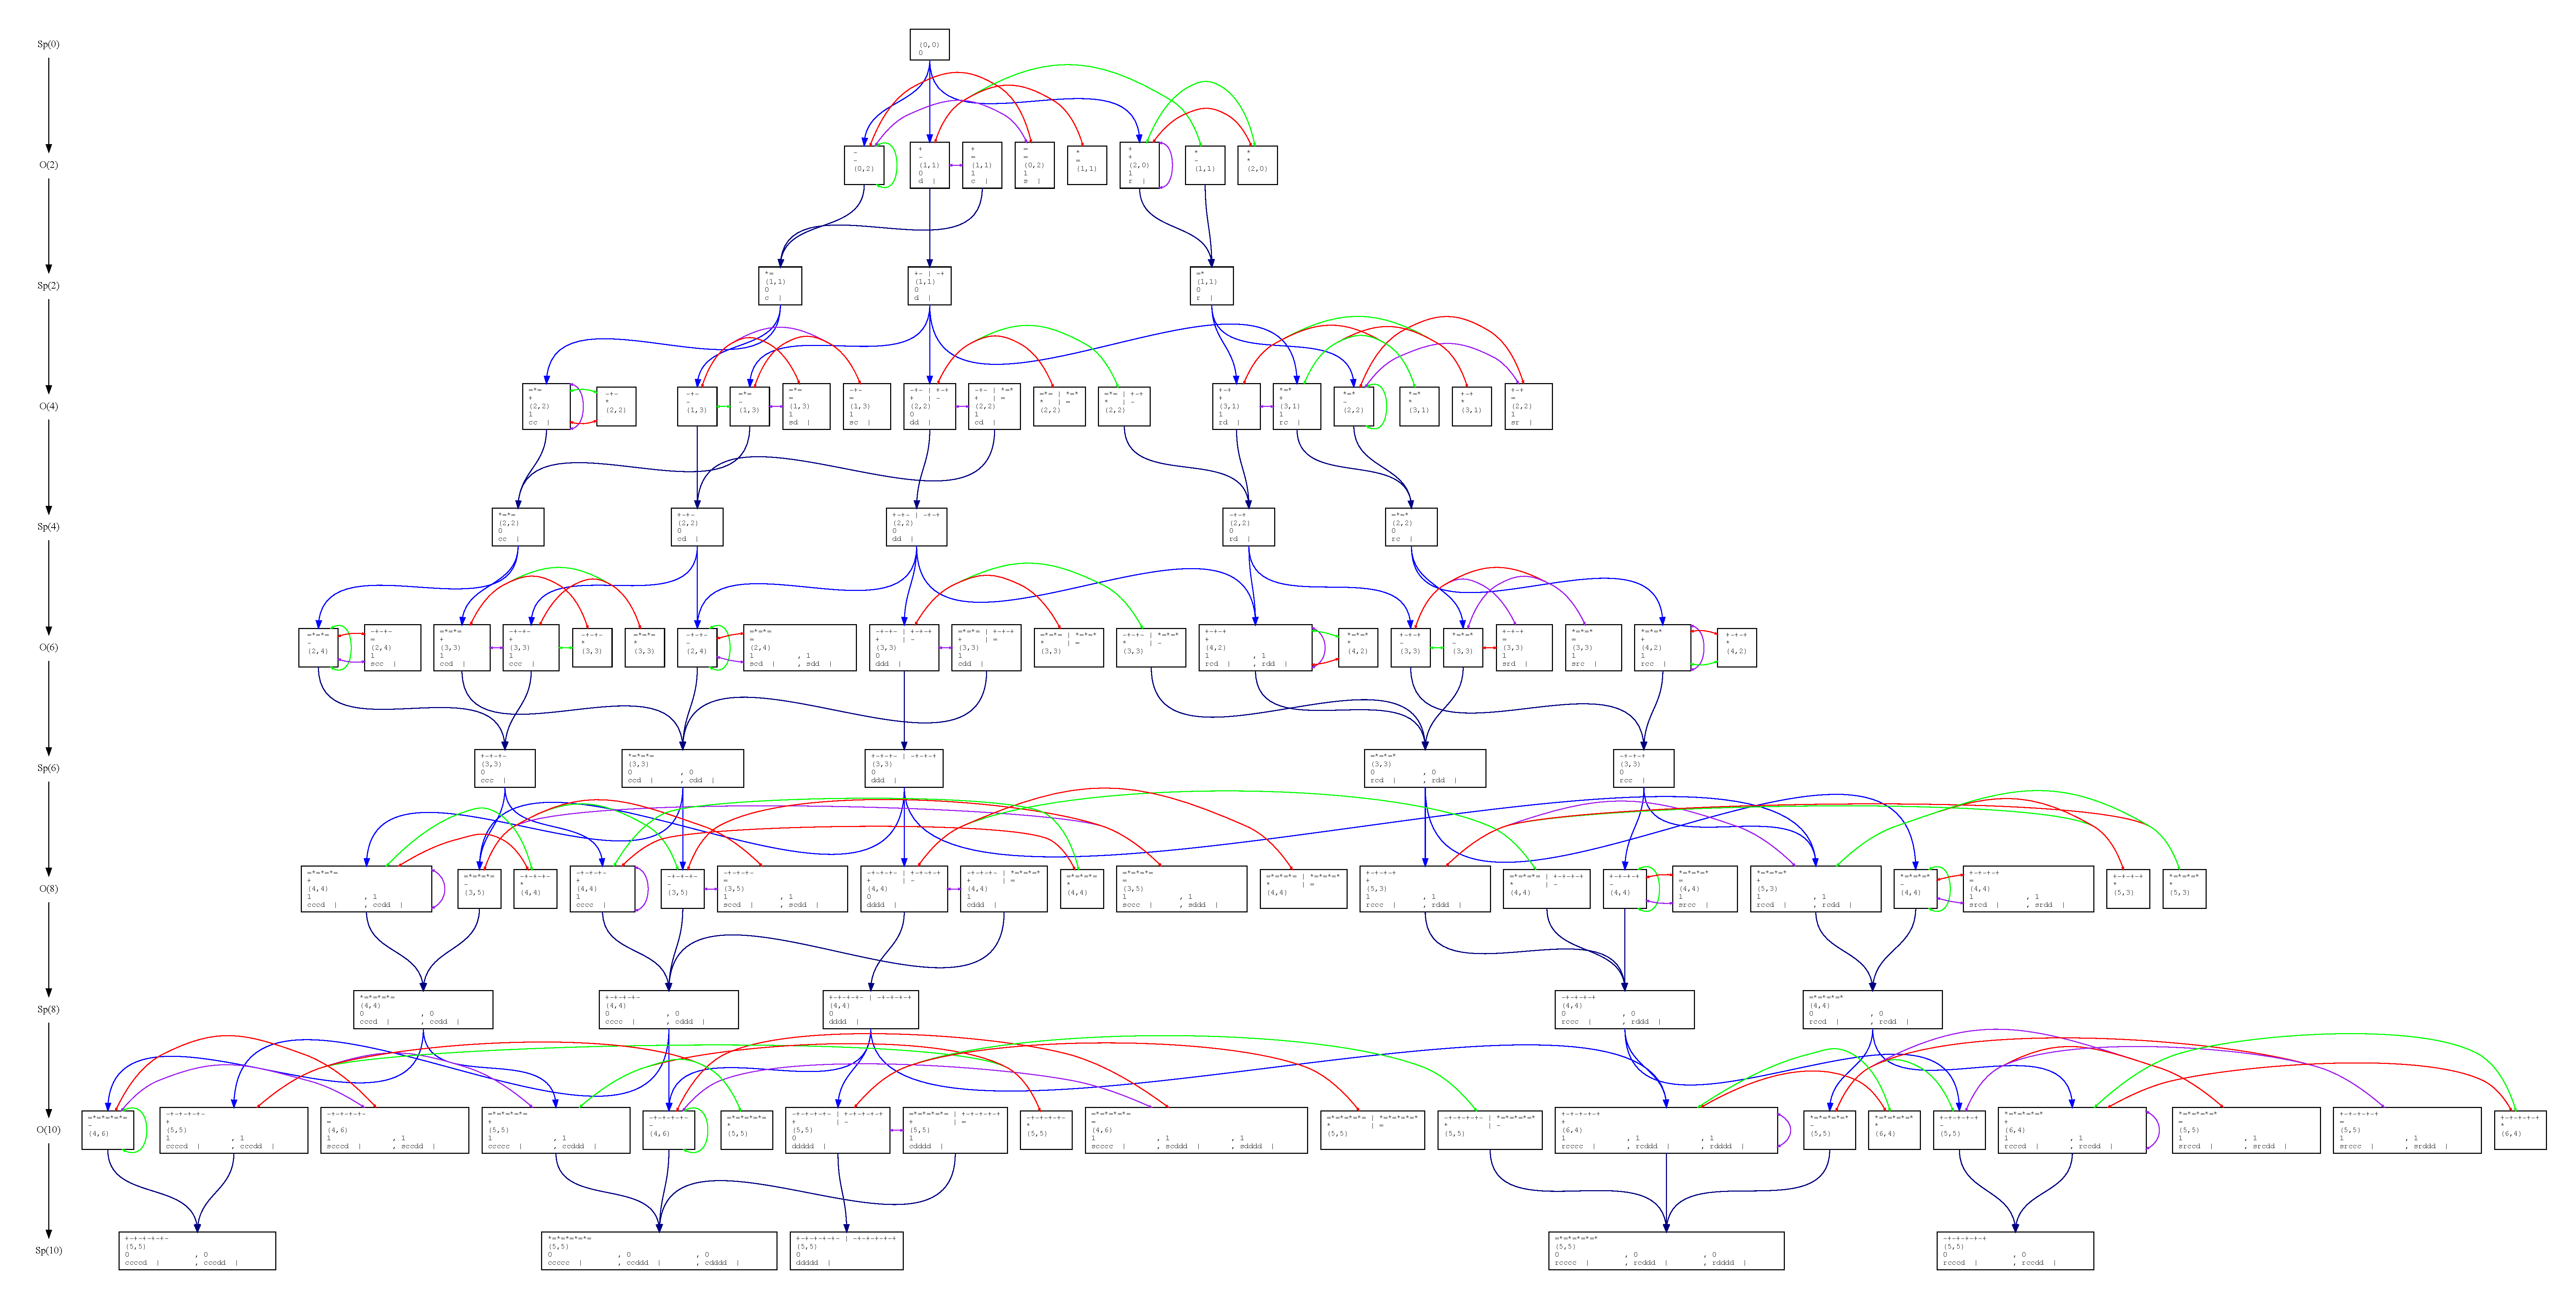
\includegraphics[width=\textwidth]{lifttreeC1_10.pdf}
      \end{frame}

  \end{document}

    \begin{frame}[label=DU]
        \frametitle{Barbasch-Vogan's definition of unipotent representation}
        \begin{itemize}[<+->]
            \item[] $G$: a real reductive group.
            \item[]  Nilpotent orbit $\ckcO$ in  
            $\bfG^\vee$.  
            \item[] \hspace{4em} $\leadsto$ $\varphi\colon \SL(2,\bC)\rightarrow \bfG^\vee$
            (Jacobson-Morozov)
            \item[] \hspace{4em} $\leadsto$ an infinitesimal character $\rdd\varphi({\half
            \tiny\begin{pmatrix} 1 & 0 \\ 0 & -1\\ \end{pmatrix} })\leftrightarrow
            \lambda_{\cO^\vee}$  
            
            \item[] \hspace{4em} $\leadsto$ the maximal primitive ideal $\cI_\ckcO$ with
            inf. char.  $\lambda_{\ckcO}$
            \item  \emph{Definition} (Barbasch-Vogan):
            \item [] An irr. admissible $G$-repn. is called 
            \emph{special unipotent} if 
            \[
            \Ann_{\cU(\fgg)}(\pi) = \cI_{\ckcO}.
            \]
            %\item  \emph{Theorem} (Barbasch-Vogan):
            \item[]
            $\Longleftrightarrow$ $\pi$ has inf. char. $\lambda_{\ckcO}$ and  
            $\AV_\bC(\pi) = \overline{\cO}$
            \item $\cO$: the  Lusztig-Spaltenstein-Barbasch-Vogan dual of $\ckcO$,
            \item[] which is a \emph{(metaplectic) special nilpotent orbit.}
            \item $\Unip_{\ckcO}(G):=$ \{ special unipotent repn. attached to $\ckcO$\}. 
        \end{itemize}
    \end{frame}


    
    \begin{frame}[label=DU]
        \frametitle{Conjecture/Open problems}
        \begin{itemize}[<+->]
            \item \emph{Major open problem:} Classify the {\red unitary dual} of a reductive group:  
            \[\whG_{\text{unitary}} = \{\text{ irr. unitary repn. of }G \}. 
            \]
            %\item[] $\Unip_{\ckcO}(G):=$ \{ special unip. repn. attached to $\ckcO$\}. 
            \item \emph{Philosophy:} $\Unip(G)=$  the {\color{red} building blocks} of the unitary dual.  
            \item \emph{Conjecture}: $\Unip_{\ckcO}(G)$ consists of {\red unitary} representations.
            %\item []  Proved by Barbasch-Vogan for complex reductive groups.`'
            \item {\red Question:} How many elements are there in $\Unip_{\ckcO}(G)$?
            \item {\red Question:} How to construct elements in $\Unip_{\ckcO}(G)$?
            \item \emph{Barbasch-Vogan} 1985: Complete classification of unipotent repn. of {\lblue complex reductive groups}. 
            \item Vogan 1986: Classify the unitary dual of {\lblue $GL(n)$}. 
            \item Barbasch 1989: Classify the unitary dual of {\lblue complex classical groups}. 
            \item \emph{Altas of Lie group:} $\leadsto$ complete answer for exceptional groups. 
        \end{itemize}
    \end{frame}
  
    % \begin{frame}{Example of Atlas' computation $G = \Sp(2,2)$}
    %     \centering{
    %     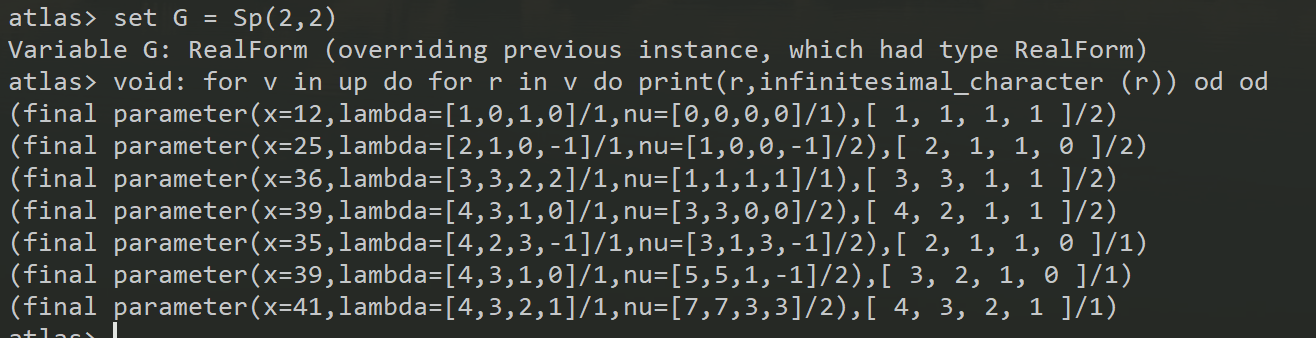
\includegraphics[width=0.8\textwidth]{atlas_Sp22.png}
    %     }
    % \end{frame}
    
    \begin{frame}[label=CT]
        \frametitle{Counting $(\fgg,K)$-module with a paticular asso. variety}
        \begin{itemize}[<+->]
            \item  Fix regular inf. char. $\lambda \in \fhh^*/W$ 
            \item  integral Weyl group
           \[
               W(\lambda) := \set{w\in W | \inn{\lambda - w\lambda}{\check\alpha}\in \bZ,
              \ \forall \alpha \in \Delta(\fgg,\fhh) 
               }
           \] 
           \item[] Double cell $\cD$  in $\widehat{W(\lambda)}$
            $\longleftrightarrow$ the specail repn. $\tau_0\in \cD$
           \item[] $\longrightarrow$ truncated induction  $J_{W(\lambda)}^W \tau_0$ 
           \item[] $\xrightarrow{\text{Springer corr.} }$ $\cO$. 
           \item Let $\mu \in \lambda + X^*$ ($X^*$ is the weight lattice), 
            \[
                W_\mu = \set{w\in W | w\cdot \mu = \mu}.  
            \]
            \item $\sG_{\lambda}(\fgg,K)$:  the Groth. gp. of $(\fgg,K)$-modules with inf. char. $\lambda$. 
            \item {\lblue Lemma: }
            \[
                \begin{split}
             & \#\set{\pi \in \Irr_{\mu}(\fgg,K)(G) | \AV_\bC(\pi) = \overline{\cO}}\\
            &= \sum_{\substack{\tau\in \cD\\\cD\leadsto \cO}} [\tau:1_{W_\mu}]\cdot [\tau: \sG_{\lambda}(\fgg,K)]
                \end{split}
            \]
        \end{itemize}
    \end{frame}

    
    \begin{frame}[label=CT]
        \frametitle{Counting unipotent representations I}
        \begin{itemize}[<+->]
            \item Example: $G = \Sp(2n,\bR)$
            \item  $\lambda_{\ckcO}\in \rho(G) + X^*$ %$\ckcO\in \Nil^{gp}(\bfG^\vee)$, i.e. $\ckcO$ only has odd length rows.  
            \item[] $\leadsto$ special representation $\tau \leftrightarrow \cO$ 
            % \item[] Springer/Lusztig left cell $\cC_\cO = \set{\tau_1,
            % \cdots,\tau_{2^l}}$ containing $\tau$
            \item $\sG_{\rho}(G)$:  the Groth. gp. of $(\fgg,K)$-modules with inf. char. $\rho$. 
            \item[]
            \vspace{-1em}
            \[
            \lblue
            \#\Unip_{\vcO}(G) = 2^l \cdot [\tau:\sG_{\rho}(G)] 
            \]
            \vspace{-1em}
            \item[] $W(\Sp(2n)) = S_n \ltimes \set{\pm 1}^n$, 
            \vspace{-1em}
            \item[] 
            \[
            \sG_{\rho}(\Sp(2n,\bR)) = \sum_{\substack{p,q,t,s,\\
            \sigma\in \widehat{S_s}}} \Ind_{S_t\times W_{2s}\times W_p\times
            W_q}^{W_n} \sgn\otimes(\sigma\times \sigma)\otimes \bfone\otimes \bfone .
            \]
            \item $[\tau:1_{W_{\lambda_{\ckcO}}}]=1$. %is counted by painted bi-partitions $\PBP(\ckcO)$.
            \item $[\tau:\sG_{\rho}(G)]$ is counted by painted bi-partitions $\PBP(\ckcO)$.
            % \item $LS(\cO)\subset \cK_\cO(\bfK)$: all local systems could be obtained by
            % theta lifting.
            % \item When $\cO^\vee\in \Nil^{qd}(\fgg^\vee)$,  $\# \PBP(\cO) 
            % = \# \AOD(\cO) = \# \LS(\cO)$ 
        \end{itemize}
    \end{frame}

    \begin{frame}{Example of $\PBP$} 
        \[
        % \lblue \ckcO = [6,6,5,5,2,2] =  \ydiagram{6,6,5,5,2,2}   
         \lblue \ckcO = [7,5,5,5,3,1,1] =  \ydiagram{7,5,5,5,3,1,1}   
        \]
        \[
        \begin{array}{ccc}
            \PBP_\ckcO(\Sp(2n,\bR)) & & \text{Associated cycle}\\
         \ytb{\bullet\bullet\bullet, \bullet c, r d, d}   
         \times 
         \ytb{\bullet\bullet\bullet, \bullet s, \none,\none}   
         & 
         \mapsto &
         \ytb{\ast=\ast=\ast=,
             \ast=\ast=\ast=,
            =\ast=\ast,
        \ast=\ast=, \ast=\ast=, -+
         }   
           \cup 
         \ytb{\ast=\ast=\ast=,
             \ast=\ast=\ast=,
            =\ast=\ast,
        =\ast=\ast, \ast=\ast=, +-
         }  \\ 
         \vdots & &\vdots 
        \end{array}
        \]
    \end{frame}


    \begin{frame}[label=CG]
        \frametitle{Nilpotent orbits with ``good/bad parity''}
        \begin{itemize}[<+->]
            \item Bad parity (must occurs with even multiplicity in $\ckcO$):
            \[
            \begin{cases}
                \text{even number,} & \text{when $\bfG^\vee$ is type $B$ or $D$}\\ 
                \text{odd number,} & \text{when $\bfG^\vee$ is type $C$} 
            \end{cases}
            \]
            \item  $\ckcO$ has \emph{``good parity'' } if $\ckcO$ only contains 
            \[
            \begin{cases}
                \text{odd rows}, & \text{when $\bfG^\vee$ is type $B$ or $D$}\\ 
                \text{even rows}, & \text{when $\bfG^\vee$ is type $C$} 
            \end{cases}
            \]
            \item $\lambda_\ckcO$ is integral.
            \item  Example of good parity:
            \[
            \begin{tikzcd}[ampersand replacement=\&,column sep=3em,row sep = -0.2em]     
                \cO \&  \vcO  \\
                \ydiagram{4,4,4,2} \& \ydiagram{5,3,3,3,1} \\  
                \Sp(14,\bC) \& \SO(15,\bC)
            \end{tikzcd} 
            \]
        \end{itemize}
    \end{frame}
    
    \begin{frame}{Reduction to the ``good parity''}
        \begin{itemize}[<+->]
            \item Consider $G= \Sp(2n,\bR)$. 
            \item  $\ckcO$ decompose into two parts $\ckcO_{g}$ (good parity)  and $\ckcO_{b}$ (bad parity).
            \item Assume $\ckcO_{b} = \{r_1, r_1, \cdots, r_k, r_k\}$.
            %  ,  $\abs{\ckcO_b}=2n_1$ and 
            % $|\ckcO_{g}| = 2n_0$
            \item[] {\lblue Theorem} (Let $\ckcO'_b = \set{r_1,\cdots, r_k}\in \Nil_{\GL}$.)
            \[
            \hspace{-2em}
            \begin{array}{ccc}
                {\tiny\Unip_{\ckcO'_b}(\GL_\bR)
                \times \Unip_{\ckcO_g}(\Sp_\bR)} &\xrightarrow{\ \ 1-1\ \ }&
                {\tiny \Unip_{\ckcO}(\Sp_\bR)} \\[.6em]
                (\pi',\pi_0 ) &\mapsto & 
                \Ind_{\raisebox{-0.5em}{\tiny$\GL(\abs{\ckcO'_b},\bR)\times \Sp(2n_0,\bR)\ltimes U$}}^{\tiny\raisebox{1em}{$\Sp(2n,\bR)$}}
                \hspace{-5em}\pi'\otimes \pi_0
            \end{array}
            \]
            \[
            \begin{split}
                {\tiny\Unip_{\ckcO'_b}(\GL)}
                = 
                \Set{\Ind \mathop{\otimes}_{j=1}^k \sgn^{\epsilon_j}_{\GL(r_j,\bR)}
                % \Set{\Ind_{\raisebox{-0.7em}{\tiny$\GL(r_1)\times\cdots\times \GL(r_k)$}}^{\tiny\raisebox{1em}{$\GL(2n_1,\bR)$}} \hspace{-6.8em}\raisebox{0em}{ $\sgn^{\epsilon_1}\otimes \cdots \otimes\sgn^{\epsilon_k}$}
                % | 
                |\epsilon_j \in \bZ/2\bZ}
            \end{split}
            \]
            \item Use \emph{theta correspondence}  to construct 
            $ \Unip_{\ckcO_{g}}(G)$.
            \item We assume  $\ckcO$ has {\red good parity} from now on.
        \end{itemize}
    \end{frame}
    
   \delete{ 
    \begin{frame}[label=CG]
        \frametitle{Construct unipotent representations by theta lifting}
        \begin{itemize}[<+->]
            \item $\bfG = \Sp(2n,\bC), \bfG^\vee = \SO(2n+1,\bC)$.
            
            \item {\lblue Good parity} orbit $\ckcO \in
            \Nil^{gp}(\fgg^\vee)\subset \Nil(\fgg^\vee)$ is an orbit satisfying
            \item []
            \vspace{-1em}
            \[
            \ckcO = (R_{2a}\geq R_{2a-3}\geq \cdots\geq R_0>0)\quad \text{all $R_i$
            are odd}
            \]
            \item {\lblue Quasi-distinguished}: 
            $R_{2i}> R_{2i-1}$ for $i = 1, \cdots, a$.  
            \item {\lblue Weakly-distinguished}: 
            $R_{2i}> R_{2i-1}$ for $i = 1, \cdots, a$.  
            \item 
            $\set{\text{good parity}}\supset \set{\text{weakly-dist.}}\supset
            \set{\text{qusi-dist.}}\supset \set{\text{dist.}}$
            \item $\leadsto$ inf. char.
            $\chi_{ \ckcO}: \cU(\fgg)^{\bfG}\rightarrow \bC$:
            \[
            \chi_{\ckcO}:= (\rho(
            R_{2a}), \rho(R_{2a-1}), \cdots, \rho(R_0), 0,  \cdots, 0 )
            \]
            where
            \[
            \rho(R):= (1, 2, \cdots, \frac{R-1}{2}).
            \]
            \item When $G = \Sp(p,q)$,  $\Unip_{\ckcO}(G) \neq  \emptyset \Longleftrightarrow $ $\ckcO$ is qusi-dist. 
        \end{itemize}
    \end{frame}
   }



    \begin{frame}[label=CG]
        \frametitle{Example of descent sequences}
        \[
        \begin{tikzcd}[ampersand replacement=\&,column sep=1em,row sep=.5em]     
            \bfG_i^\vee \&  \SO(15,\bC) \&  \rO(10,\bC) \&  \SO(7,\bC) \& \rO(4,\bC)\\
            \vcO_i \& \ydiagram{5,3,3,3,1} \&
            \ydiagram{0,3,3,3,1} \& \ydiagram{0,0,3,3,1} \& \ydiagram{0,0,0,3,1}    \\
            \cO_i \& \ydiagram{4,4,4,2}\& \ydiagram{3,3,3,1} \& \ydiagram{2,2,2,0} \&
            \ydiagram{1,1,1,1}\\
            \bfG_i \&  \Sp(14,\bC) \&  \rO(10,\bC) \&  \Sp(6,\bC) \& \rO(4,\bC)\\
        \end{tikzcd} 
        \]
        \pause

        {\lblue Kraft-Procesi's} resolution  of singularities of the closure of complex nilpotent orbits. 
    \end{frame}
    
    \begin{frame}[label=CG]
        \frametitle{Descent of nilpotent orbits: $G = \Sp(2n,\bR)$ }
        \begin{itemize}[<+->]
            \item 
            Take $\ckcO\in \Nil^{gp}(\fgg^\vee)$ (nilpotent orbits with good parity).
            \item
            {\lblue Descent sequence on the dual side:}  
            \vspace{-1em}
            \[
            \begin{tikzcd}[ampersand replacement=\&,column sep=1em]
                \vcO =\vcO_{2a} \&  \vcO_{2a-1} \& \cdots \& \vcO_0
            \end{tikzcd}
            \]
            \vspace{-2em}
            \item[] $\vcO_i =$  removing the first rows of $\vcO_{i+1}$.
            \item
            {\lblue 
            Descent sequence of real classical groups:} 
            \vspace{-1em}
            \[
            \begin{tikzcd}[ampersand replacement=\&,column sep=1em]
                G = G_{2a} \&  G_{2a-1} \& \cdots \& G_{0} 
            \end{tikzcd}
            \]
            \vspace{-2em}
            \begin{itemize}
                \item $G_{2k}$ is a symplectic group
                \item[] allow $G_0 = \Sp(0,\bR)=$ the trivial group.
                \item $G_{2k-1} = \rO(p_k,q_k)$
                \item $\vcO_i$ is nilpotent orbit of $\bfG^\vee_{i}$
            \end{itemize}
            \item  $(G_i,G_{i-1})$ forms a reductive dual pair.
            \item $\cO_i = $ delete the first col.  of $\cO_{i+1}$ 
            and may add one box back. %to the remaining longest column making the size correct. 
        \end{itemize}
    \end{frame}
    
    
    \begin{frame}[label=CG]
        \frametitle{Example of descent sequences}
        \[
        \begin{tikzcd}[ampersand replacement=\&,column sep=1em,row sep=.5em]     
            \bfG_i^\vee \&  \SO(15,\bC) \&  \rO(10,\bC) \&  \SO(7,\bC) \& \rO(4,\bC)\\
            \vcO_i \& \ydiagram{5,3,3,3,1} \&
            \ydiagram{0,3,3,3,1} \& \ydiagram{0,0,3,3,1} \& \ydiagram{0,0,0,3,1}    \\
            \cO_i \& \ytb{-+-+\none,+-+-,+-+-,+-}\& \ytb{+-+,-+-,-+-,-} \& \ytb{-+\none,+-,+-,\none} \&
            \ytb{+,+,-,-\none\none}\\
            G_i \&  \Sp(14,\bR) \&  \rO(4,6) \&  \Sp(6,\bR) \& \rO(2,2)\\
        \end{tikzcd} 
        \]
        \pause
        {\lblue Ohta's} resolution  of singularities of a nilpotent orbit closure in symmetric pairs. 
    \end{frame}
    
    
    \begin{frame}[label=CG]
        \frametitle{Construction of elements in $\Unip_{\ckcO}(G)$}
        \begin{itemize}[<+->]
            \item 
            $\chi=\displaystyle\mathop{\otimes}_{j=0}^{2a}\chi_{j}$, a 1-dim repn. 
            of
            $\displaystyle\mathop{\textstyle\prod}_{j=0}^{2a}G_{j}$.
            \item $\chi_j \in \{ \bfone, \sgn^{+,-}, \sgn^{-,+},  {\det}\}$
            \item 
            Define a smooth repn. of $G = G_{2a}$ (the symplectic group). 
            \[
            {\lblue \pi_{\chi}}:=(\omega_{G_{2a},G_{2a-1}}\widehat \otimes
            \omega_{G_{2a-1},G_{2a-2}} \widehat \otimes \cdots \widehat \otimes
            \omega_{G_1,G_0} \otimes \chi)_{G_{2a-1}\times G_{2a-2}\times \cdots \times G_{0}}
            \]
            \item[]
            \begin{thm}[Barbasch-M.-Sun-Zhu]
                Let  $\ckcO^\vee$ be an orbit with good parity.
                Then
                \begin{itemize}[<+->]
                    \item either $\pi_\chi = 0$ or
                    \item $\lblue \pi_{\chi}\in  \Unip_{\ckcO}(G)$ and   
                    {\lblue unitarizable}.
                    \item Moreover, 
                    \[\lblue
                    \Unip_{\vcO}(G) = \set{\pi_{\chi} | \pi_{\chi}\neq 0}. 
                    \]
                \end{itemize}
            \end{thm}
        \end{itemize}
    \end{frame}
    
    
    
    \begin{frame}[label=CT]
        \frametitle{Example: Coincidences of theta lifting}
        Lift to $G = \Sp(6,\bR)$ from real forms of $\bfG = \rO(4,\bC)$.\\
        $\ckcO = 3^2 1^1$ and  $\cO = 2^3$.
        \[
        \begin{tikzcd}[ampersand replacement=\&,column sep=2em, row sep=1em]
            \& \& \Sp(6,\bR)\\
            %\hline
            \rO(4,0) \& \  \& \theta(\sgn^{+,-}) \ar[dr,equal]\& \   \\
            \rO(3,1) \& \theta(\bfone) \& \theta(\sgn^{+,-}) \ar[dr,equal] \& \theta(\sgn^{-,+}) \\
            \rO(2,2) \& \theta(\bfone) \& \theta(\sgn^{+,-}) \ar[dr,equal] \& \theta(\sgn^{-,+}) \\
            \rO(1,3) \& \theta(\bfone) \& \theta(\sgn^{+,-}) \ar[dr,equal] \& \theta(\sgn^{-,+}) \\
            \rO(0,4) \& \  \&\  \& \theta(\sgn^{-,+}) \\
        \end{tikzcd}
        \]
    \end{frame}
    
    
    
    
    \begin{frame}[label=CG]
        \frametitle{Some comments}
        \begin{itemize}[<+->]
            \item Many people have studied the problem
            \item[] Adams, Barbasch,  He, Huang, Li, Loke, M\oe glin, Paul, Przebinda, Trapa,  ....
            \item {\lblue Unitarity}:
            \begin{itemize}
                \item Estimate of matrix coefficients using the explicit realization of the
                Weil representations.
                \item[] Work of {\bf Li}, {\bf He}, and an idea of {\bf Harris-Li-Sun} showing
                the {\lblue nonnegativity} of a matrix coefficient integral.
            \end{itemize}
            \item {\lblue non-vanishing} and compute {\lblue associated cycle}:
            \begin{itemize}
                \item {\bf Geometry}: moment maps provide the \underline{upper bound}.
                \item {\bf Analysis}: degenerate principal series force the \underline{lower
                bound}.
                \item {\bf Geometry meets Analysis}: the equality.
            \end{itemize}
            \item {\lblue Exhaustion:} Combinatorics  {\red (recent breakthrough!)} 
            \item {\lblue Corollary:} (using [Gomez-Zhu]) For $\pi_\chi$, 
           \[
            \text{Whittaker cycle   = Wavefront cycle. }
           \] 
            
        \end{itemize}
    \end{frame}
    



\begin{frame}[label=AC]
  %\frametitle{Geometry of the \underline{moment maps}}
  \frametitle{Associated cycle formula I}
  \begin{itemize}[<+->]
  \item Example $(G,G')=(\Sp(2n,\bR), \rO(p,q))$ 
    \[
      \begin{tikzcd}[ampersand replacement=\&,column sep=3em, row sep=1em]
        \& M_{p,n}\oplus M_{q,n} \ar[rd,"\varphi"]
        \ar[ld,"\varphi'"'] \& \\
        M_{p,q}\cong {\mathfrak{p}'} \&  \text{\footnotesize $(A,B)$} \ar[rd,mapsto]\ar[ld,mapsto]\& {\mathfrak p}\cong
        \mathrm{Sym}_n\oplus \mathrm{Sym}_n\\
       \text{\footnotesize $X'=AB^T$} \& \& \text{\footnotesize $X = (A^T A,B^T B)$} \\
      \end{tikzcd}
    \]
  \item $\bcO \cap \fpp \supset \varphi(\varphi'^{-1}(\fpp'\cap \cO'))$ where
    $\cO$ is a cplx. nil. $\bfG$-orbit. 
  \item {\lblue Upper bound} of associated cycle: we can define 
  \item[]
    \[\vartheta^{\text{geo}}\colon
       \cK_{\cO'}(G') \longrightarrow \cK_{\cO}(G)\]
   \item[] such that
    \[
       \AC(\Theta(\pi'))\preceq \vartheta^{\text{geo}} (\AC(\pi')),
     \]
     for any $\pi'$ with $\AV(\pi')\subset \overline{\cO'}$
  \end{itemize}
\end{frame}

\begin{frame}[label=AC]
  \frametitle{Associated cycle formula II}
  \begin{itemize}[<+->]
  \item Recall 
    $(G,G')=(\Sp(2n,\bR), \rO(p,q))$
  \item For $\sL' \in \cK_{\cO'}(G')$, $\sL = \vartheta(\sL')\in \cK_{\cO}(G)$,
    \[
      \sL_X = \vartheta_{T}(\sL_{X'}):= {\red {\det}^{(p-q)/2}|_{K_{X}}} 
     \otimes (\sL'_{X'})^{K'_{2,X'}} \circ \alpha,
    \]
  \item[] $\alpha\colon K_X \longrightarrow K'_{1,X'}$:
     a homomorphism between isotropic subgroups.
  \item The twisting is {\lblue crucial}. 
  \item[] $\Rightarrow$ {\lblue admissible orbit data $\leadsto$ admissible orbit data. }

  \item Support of $\vartheta(\sL')$ could be reducible. 

  \item Stable range lifting trick: Suppose $n > p+q$. 
    \[
      \bigcup_{p,q}\Unip_{\cO^{'\vee}}(\rO(p,q)) \hookrightarrow \Unip_{\vcO}(\Sp(2n,\bR))
    \]
  \end{itemize}
\end{frame} 


    
    % \begin{frame}[label=CT]
    %     \frametitle{Counting unipotent representations I}
    %     \begin{itemize}[<+->]
    %         \item  $\ckcO\in \Nil^{gp}(\bfG^\vee)$ 
    %         \item[] $\leadsto$ special representation $\tau \leftrightarrow \cO$
            
    %         % \item[] Springer/Lusztig left cell $\cC_\cO = \set{\tau_1,
    %         % \cdots,\tau_{2^l}}$ containing $\tau$
    %         \item $\sG_{\rho}(G)$:  the Groth. gp. of $(\fgg,K)$-modules with
    %         inf. char. $\rho$. 
    %         \item[]
    %         \vspace{-1em}
    %         \[
    %         \lblue
    %         \#\Unip_{\vcO}(G) = 2^l \cdot [\tau:\cK_{\rho}(G)] 
    %         \]
    %         \vspace{-1em}
    %         \item[] $W(\Sp(2n)) = S_n \ltimes \set{\pm 1}^n$, 
    %         \vspace{-1em}
    %         \item[] 
    %         \[
    %         \sG_{\rho}(\Sp(2n,\bR)) = \sum_{\substack{p,q,t,s,\\
    %         \sigma\in \widehat{S_s}}} \Ind_{S_t\times W_{2s}\times W_p\times
    %         W_q}^{W_n} \sgn\otimes(\sigma\times \sigma)\otimes \bfone\otimes \bfone .
    %         \]
    %         \item $[\tau:\sG_{\rho}(G)]$ is counted by painted bi-partitions
    %         $\PBP(\ckcO)$.
    %         % \item $LS(\cO)\subset \cK_\cO(\bfK)$: all local systems could be
    %         % obtained by theta lifting. \item When $\cO^\vee\in
    %         % \Nil^{qd}(\fgg^\vee)$,  $\# \PBP(\cO) = \# \AOD(\cO) = \#
    %         % \LS(\cO)$ 
    %     \end{itemize}
    % \end{frame}

    \begin{frame}[label=CT]
        \frametitle{Matching unipotent representations with PBP}
        \begin{itemize}[<+->]
            \item $\PBP(\ckcO)$ is complicate.
            \item $\LS(\ckcO) = \set{\AC(\pi_\chi)}$ is also complicate.
            \item {\lblue Proof of Exhaustion}
            \item[] Define descent of painted bi-partitions, 
            \item[] {\red compatible with the theta lifting!}
            \[
            \begin{tikzcd}[ampersand replacement=\&]
               \LS(\ckcO) \& \PBP(\ckcO) \ar[r,<->]\ar[d,"\nabla"'] \ar[l,"\AC"]\& \Unip_{\ckcO}(G)  \\
               \LS(\ckcO') \ar[u,"\vartheta^{\text{geo}}"]\& \PBP(\ckcO') \ar[r,<->]\ar[l,"\AC"] \& \Unip_{\ckcO'}(G') \ar[u,"\theta"'] 
            \end{tikzcd}
            \]
            \item[] 
            \[
                \pi_{\tau} := \Theta(\pi_{\nabla(\tau)}\otimes \chi'_{\tau})\otimes \chi_{\tau}
            \]
            \item The {\red injectivity} of theta lifting is crucial!
        \end{itemize}
    \end{frame}
    


    % \begin{frame}
    % \frametitle{More precise statement}

    % \end{frame}
   
        % \begin{frame}{Example: $\cO=$ regular nilpotent orbit}
        %    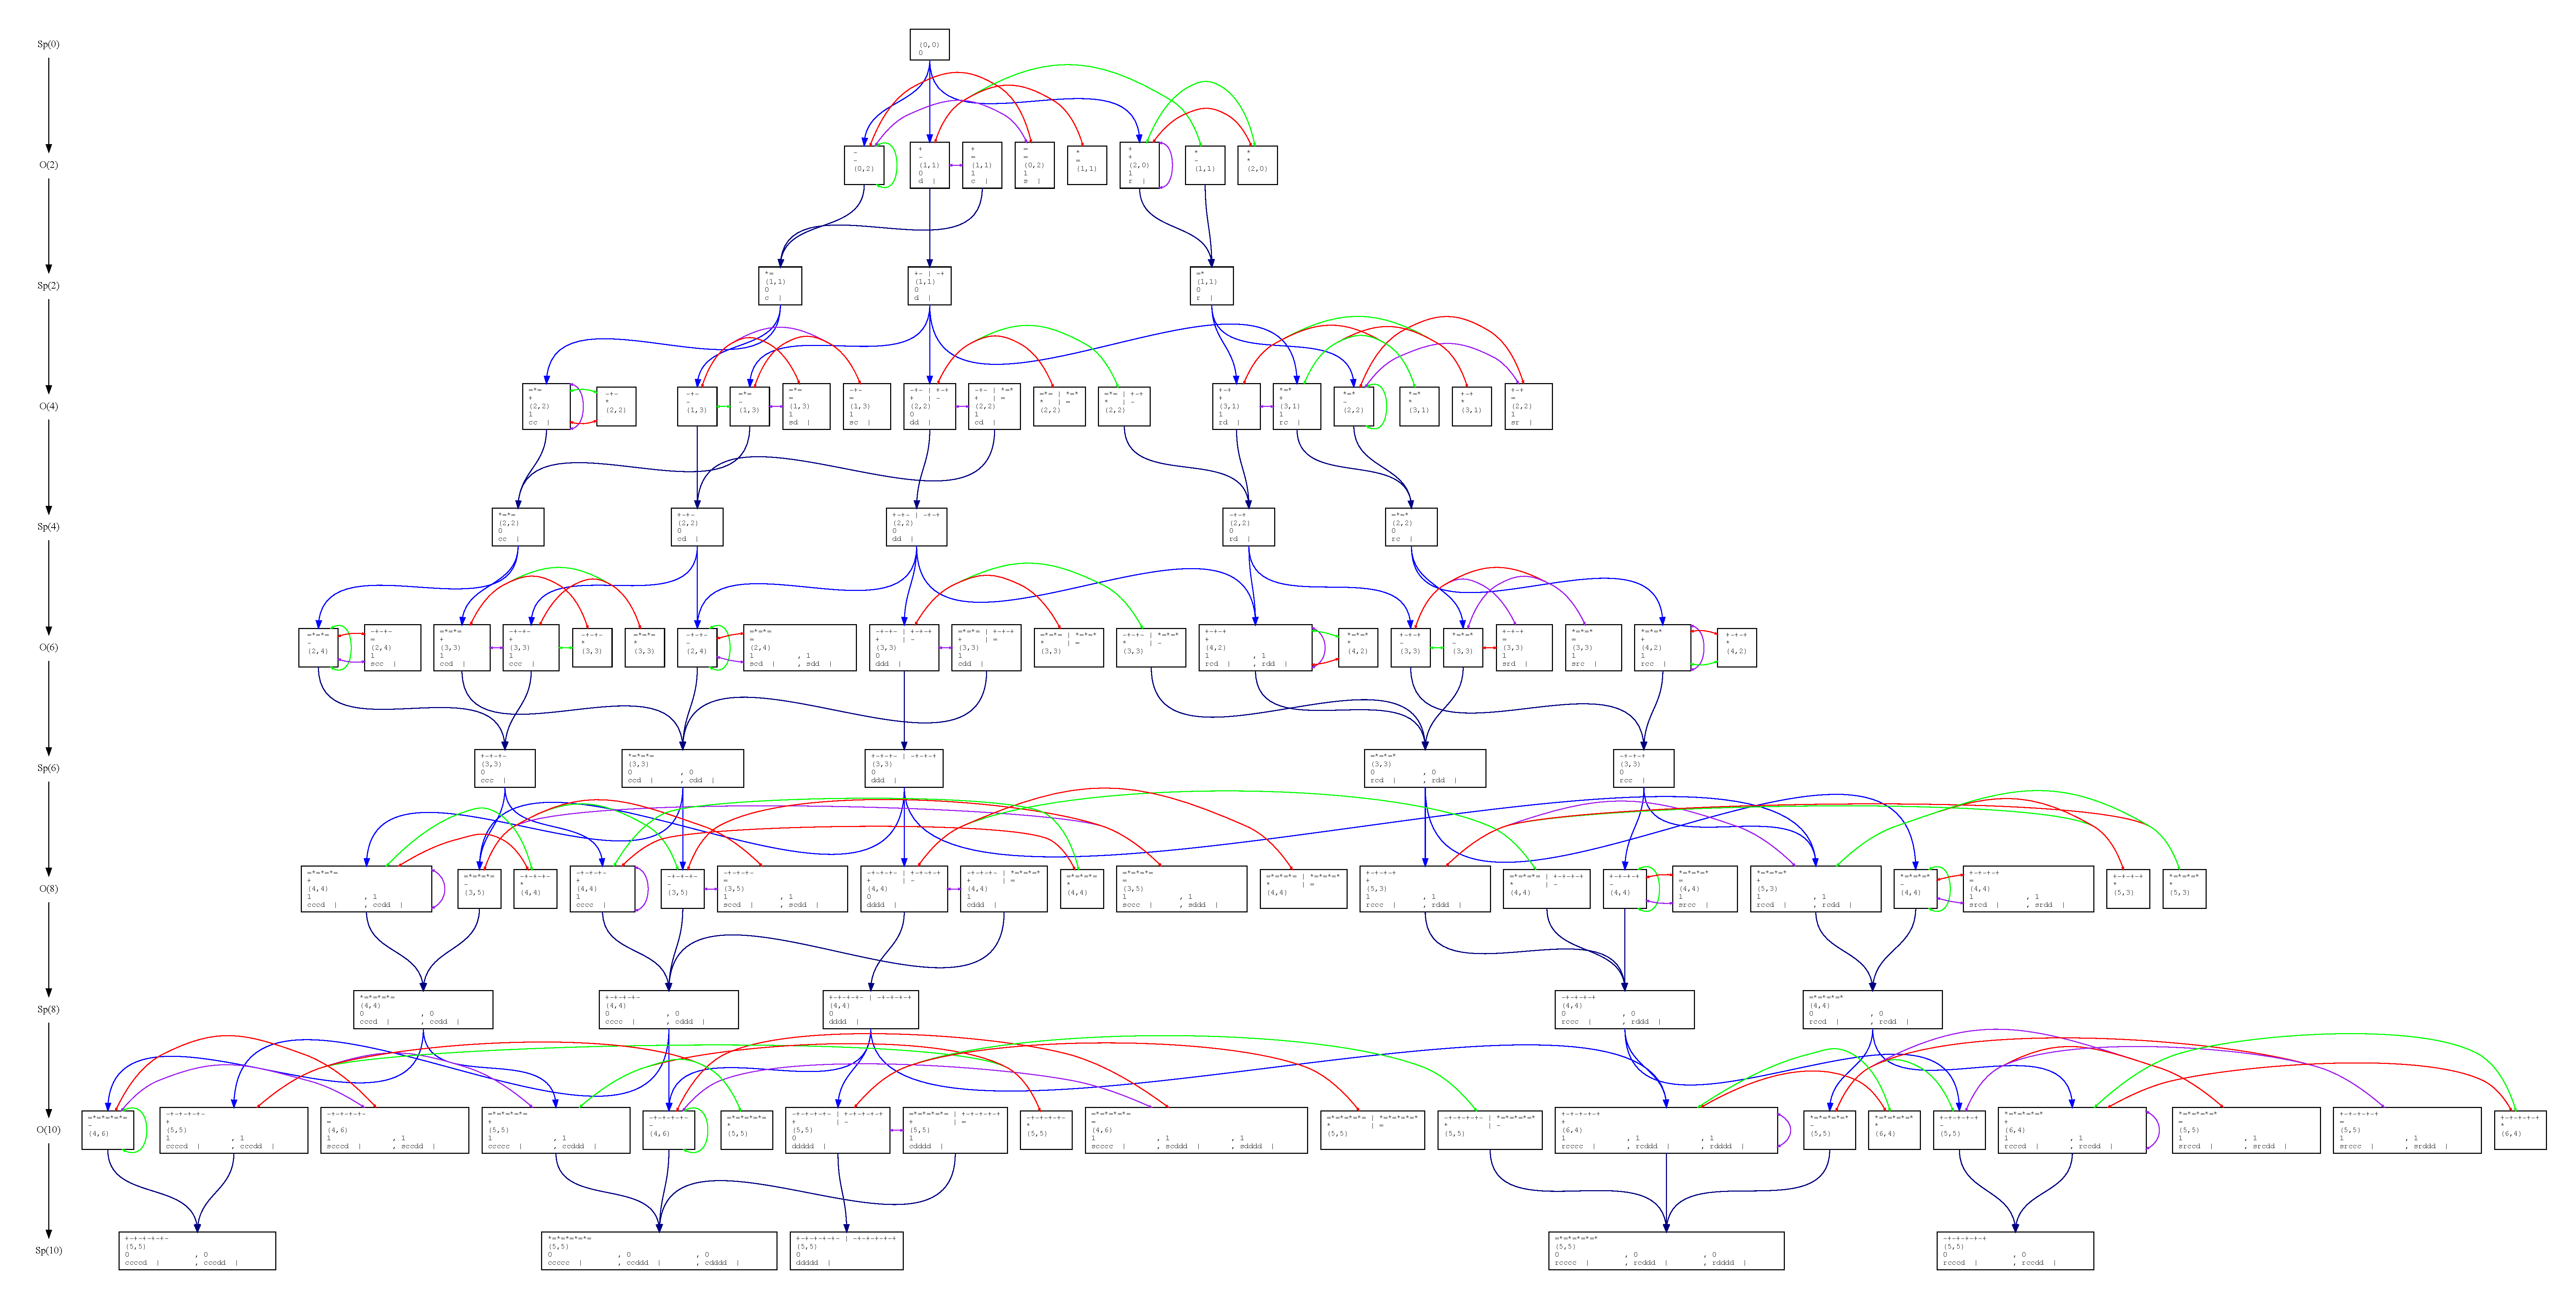
\includegraphics[width=\textwidth]{lifttreeC1_10.pdf}
        % \end{frame}

    \begin{frame}[label=DU]
        \frametitle{Unipotent Arthur packet}
        
        \begin{itemize}[<+->]
            \item {\lblue Arthur parameter:}
            $\psi\colon W_\bR\times \SL_2(\bC)\rightarrow \bfG^\vee \rtimes \Gal(\bC/\bR)$.
            
            \item[]\hspace{4em} Here $W_\bR = \bC\rtimes \langle j\rangle $.
            \item Arthur's Arthur packet $\Pi_{\psi}^{A}(G)$:
            \item[] \hspace{2em} \{local components of automorphic
            cusp. repn. \}
            \item[] {\red They are unitary by definition!}
            \item {\lblue Unipotent Arthur parameter}: $\psi|_{\bC^\times}$ is trivial.
            \item[]  M\oe glin: $\pi_{\psi, \eta}$ is zero or multiplicity free ($\eta\in\Irr(\pi_1(Z_{\bfG^\vee}(\psi)))$). 
            \item[] {\lblue Warning:} {\red  $\Pi_{\psi}^A(G) \cap
            \Pi^A_{\psi'}(G)\neq \emptyset$ } in general.
            \item {\lblue ``Corollary'':}
            \[
            \Pi_{\psi}^{A}(G) = \Pi_{\psi}^{ABV}(G) 
            \]
            \item {\lblue Question:} How to  describe $\pi_{\psi,\eta}$ explicitly?  
        \end{itemize}
    \end{frame}
    
    
    
    \begin{frame}
        \vfill
        %\centering{\bf\Large {\tt{atlas}} is a great teacher!} \\
        %\vspace{2em}
        %\pause
        %\centering{\bf\Large Thanks to the {\tt{atlas}} team!} \\
        %\pause
        %\vspace{2em}
        Dan Barabasch, M. ,  Binyong Sun and Chen-Bo Zhu\\
        Special unipotent representations: orthogonal and symplectic groups\\
         ArXiv e-prints: \href{https://arxiv.org/abs/1712.05552v2}{https://arxiv.org/abs/1712.05552v2}
       \vfill 
        \centering{\bf\Large\color{blue} Thank you for your attention!}
        \vfill
         
\includegraphics[width=.3\textwidth]{arxiv_uni.png}
    \end{frame}
    
    \end{document}
    
    


%%% Local Variables: 
%%% coding: utf-8
%%% mode: latex
%%% TeX-engine: xetex
%%% TeX-master: t
%%% End:
